\chapter{Background and related work}
\label{chap:literature_review}

Methods for longitudinal causal inference can be organized along two main dimensions: 
the structure of the causal diagram and the causal target of interest. 
The structure of the causal setting is typically represented by a directed acyclic graph (DAG) 
that encodes the assumptions about the data generating process and the causal relationships 
between the variables \cite{pearlCausalityModelsReasoning2009}. The presence or absence of 
treatment-confounder feedback 
and unobserved confounders are important features of the causal structure that can affect the 
choice of estimation method. The causal target of interest, on the other hand, is driven by the 
research question and scientific context of the study \cite{lundbergWhatYourEstimand2021}. Different methods may be designed to estimate 
different causal targets, such as the average treatment effect at a specific time point, the cumulative 
effect of treatment over time, or the contrast between two specific treatment regime. Having these 
two dimensions in mind, in the 
following sections, we will review the relevant literature on longitudinal causal inference 
and the methods exist to address confounding.

\section{Potential outcomes and treatment regimes}
The causal targets are often formalized in the potential-outcomes framework \cite{rubinEstimatingCausalEffects1974}. 
In this framework, we define the potential outcome of individual $i$ as $Y_i(a)$, representing the outcome that would be observed if 
the treatment $A$ were set to a specific value $a$. Note the difference between the observed outcome $Y_i$ and the 
potential outcome $Y_i(a)$ which is an unobserved variable, 
as we can only observe the outcome under the treatment that was actually assigned to. Similarly, in the longitudinal setting, we can define the potential outcome at time $t$ for a 
static\footnote{The static here is to contrast with a 
dynamic treatment regime, where treatments depends on the values of the confounders \cite{moodieDemystifyingOptimalDynamic2007}. In this thesis we only consider static treatment regimes.} treatment regime 
$\bar{a}_t = (a_0, a_1, a_2, \ldots, a_t)$ as $Y_{i,t+1}(\bar{a}_t)$, 
representing the outcome that would be observed if the treatment were set to specific values at each 
time point. In a similar way, the 
potential value of confounders at time $t$ can also be defined as $X_{i,t}(\bar{a}_{t-1})$, 
representing the value of the confounder at time $t$ that would be observed if the treatment 
were set to specific values at each time point up to $t-1$\footnote{Here we follow the Robins indexing convention to emphasize the temporal ordering of the treatments, 
confounders and (repeated) outcome \cite{hernanCausalInferenceWhat2023}. Counfounders at time time $t$ is measured after the treatment at time $t-1$ 
and before the treatment at time $t$. Moreover, the potential outcome is indexed at time $t+1$ to reflect 
the fact that the outcome is determined after the treatment while the measured outcome at time $t$ may act 
as a confounder for the treatment at time $t$ and the outcomes at later time points.}.

\section{Treatment-confounder feedback}
Treatment-confounder feedback occurs when the treatment at time $t$ can affect the confounders at later 
time points. This creates a feedback loop between the treatment and the confounders, 
which can lead to bias if not properly adjusted for. in Figure \ref{fig:sample_dags} (b), these feedback loops 
are represented by the purple arrows from $A_t$ to subsequent $X_{t+k}$ where $1 \le k \le T-k$. These structures 
are problematic for standard regression-based methods, as they can lead to collider 
bias if we condition on the confounders at time $t$; And the confounder 
\section{Identification under sequential ignorability}
There are well-established methods for 
identifying and estimating the average potential outcomes of statatic treatment regimes when treatment-confounder feedback is present.
These methods—known as the g-methods—include the g-formula \cite{robinsEstimationCausalEffects2008,snowdenImplementationGComputationSimulated2011}, marginal structural models (MSMs) \cite{robinsMarginalStructuralModels2000}, 
and structural nested models (SNMs) \cite{vansteelandtStructuralNestedModels2014}. 
They all rely on the assumption of sequential ignorability, 
which states that the potential outcomes 
\section{Treatment-confounder feedback}
\begin{comment}  
Longitudinal causal inference is a broad area of research with a rich literature. There are 
two main dimensions along which the longitudinal causal estimators can be organized. The first is the structure 
of the causal setting, typically represented by a directed acyclic graph (DAG) 
with a set of nodes $\mathbf{V}$ and a set of directed edges $\mathbf{E}$. 
Each node in the graph represents a variable and each directed edge 
represents a causal relationship between two variables. 
The structure of the causal diagram encodes the assumptions about the 
data generating process and the causal relationships between the variables \cite{pearlCausalityModelsReasoning2009}. This includes 
features such as the presence or absence of treatment-confounder feedback or presence 
of unobserved confounders as shown in Figure \ref{fig:sample_dags}. Some methods are designed to work in specific types 
of causal structures, while others are more general and can be applied to a wider range of settings.


The second dimension is about the causal target of interest, that is, the 
estimand addressed by the method. This dimension is driven by the research question and 
the scientific context of the study \cite{lundbergWhatYourEstimand2021}. 
For example, in a longitudinal study with time-varying treatments, 
one might be interested in estimating the average treatment effect at a specific time point, 
the cumulative effect of the treatment over time, or the effect of a specific treatment regime. A particular method 
might be able to estimate one or more of these targets, but not all of them.


\section{Setup and causal estimands in longitudinal studies}
\subsection{Potential outcomes under static and dynamic treatment regimes}
The causal targets are often formalized in the potential-outcomes framework \cite{rubinEstimatingCausalEffects1974}. 
In this framework, we define the potential outcome of individual $i$ as $Y_i(a)$, representing the outcome that would be observed if 
the treatment $A$ were set to a specific value $a$. Then one common causal target, the average treatment effect (ATE), is defined as 
the difference in expected potential outcomes under different treatment values, i.e., $\text{ATE} = \mathbb{E}[Y_i(1) - Y_i(0)]$ 
for a binary treatment. Note the difference between the observed outcome $Y_i$ and the 
potential outcome $Y_i(a)$ which is an unobserved variable, 
as we can only observe the outcome under the treatment that was actually assigned to.

Similarly, in the longitudinal setting, we can define the potential outcome at time $t$ for a 
\emph{static} treatment regime 
$\bar{a}_t = (a_1, a_2, \ldots, a_t)$ as $Y_{i,t+1}(\bar{a}_t)$, 
representing the outcome that would be observed if the treatment were set to specific values at each 
time point. In a similar way, the 
potential value of confounders at time $t$ can also be defined as $X_{i,t}(\bar{a}_{t-1})$, 
representing the value of the confounder at time $t$ that would be observed if the treatment 
were set to specific values at each time point up to $t-1$. The static here is to contrast with a 
\emph{dynamic} treatment regime, where treatments depends on the values of the confounders \cite{moodieDemystifyingOptimalDynamic2007}. 

\subsection{Treatment-confounder feedback and temporal ordering}

Here we follow the Robins style of indexing convention to emphasize the temporal ordering of the treatments, 
confounders and (repeated) outcome \cite{hernanCausalInferenceWhat2023}. Counfounders at time time $t$ is measured after the treatment at time $t-1$ 
and before the treatment at time $t$. Moreover, the potential outcome is indexed at time $t+1$ to reflect 
the fact that the outcome is determined after the treatment while the measured outcome at time $t$ may act 
as a confounder for the treatment at time $t$ and the outcomes at later time points. 
\end{comment}

\section{Identification under sequential ignorability}
When all confounders are measured, there are well-established methods for 
identifying and estimating causal effects in longitudinal settings. 
These methods include g-methods such as the g-formula \cite{robinsEstimationCausalEffects2008}, marginal structural models (MSMs) \cite{robinsMarginalStructuralModels2000}, and structural nested models (SNMs) \cite{vansteelandtStructuralNestedModels2014}. 
These methods rely on the assumption of sequential ignorability, 
which states that there are no unmeasured confounders at each time point.

methods to deal with unmeasured confounding can be divided based on how they 
deal with the sequential ignorability assumption. some methods such as the deconfounder 
methods try to retain the sequential ignorability assumption by estimating a substitute 
for the unmeasured confounders, 
while FE-MSM assume a version of sequential ignorability that is conditional on the unit-specific unobserved heterogeneity component, 
while other methods such as instrumental variable methods or proxy variable methods try to relax the 
sequential ignorability assumption by using additional data with a specific structure.

\subsection{G-methods}
\cite{vansteelandtStructuralNestedModels2014}
\cite{robinsEstimationCausalEffects2008}
\cite{keilParametricGformulaTimetoevent2014}

\subsubsection{Marginal structural models}
\cite{robinsMarginalStructuralModels2000}
\cite{neugebauerCausalInferenceLongitudinal2007}


\section{Methods for unmeasured confounding in longitudinal settings}
\subsection{Time-invariant unmeasured confounding and panel structure}
\cite{imaiWhenShouldWe2019} -> \cite{blackwellEffectPoliticalAdvertising2024} 

\subsection{Latent-variable approaches}
\cite{wangBlessingsMultipleCauses2019}
\cite{bicaTimeSeriesDeconfounder2020}
\cite{hattSequentialDeconfoundingCausal2024}

\subsection{Proximal causal inference}
\cite{tchetgenIntroductionProximalCausal2020} -> \cite{yingProximalCausalInference2023}, \cite{deanerProxyControlsPanel2023}


\subsection{Instrumental-variable approaches for longitudinal unmeasured confounding}
\cite{angristIdentificationCausalEffects1996} -> \cite{michaelInstrumentalVariableEstimation2020} ->\cite{chengInstrumentalVariableEstimation2024}





There are different causal targets that can be defined in the longitudinal setting. A  
 such as the average treatment effect at time $t$, the cumulative effect of the treatment over time, or the effect of a specific treatment regime. The choice of the causal target depends on the research question and the scientific context of the study. For example, if we are interested in the effect of a treatment at a specific time point, we might focus on estimating the average treatment effect at that time point. If we are interested in the overall effect of a treatment over time, we might focus on estimating the cumulative effect of the treatment. If we are interested in the effect of a specific treatment regime, we might focus on estimating the effect of that regime compared to another regime.
This inde that the potential outcome is defined at time $t+1$ 
to emphasize that the outcome is determined after the treatment at time $t$, where the treatment at time $t$ can affect the confounders at later time points.
The average treatment effect at time $t$ can then be defined as $\text{ATE}_t = \mathbb{E}[Y_{i,t+1}(\bar{a}_t) - Y_{i,t+1}(\bar{a}'_t)]$ for two different treatment regimes $\bar{a}_t$ and $\bar{a}'_t$.
as $Y_i(a_1, a_2, \ldots, a_t)$, representing the outcome that would be observed if the treatment were set to specific values at each time point. The average treatment effect at time $t$ can then be defined as $\text{ATE}_t = \mathbb{E}[Y_i(a_1, a_2, \ldots, a_t) - Y_i(a'_1, a'_2, \ldots, a'_t)]$ for two different treatment regimes.




\begin{figure}[htbp]
\centering

\begin{subfigure}{0.8\textwidth}
\centering
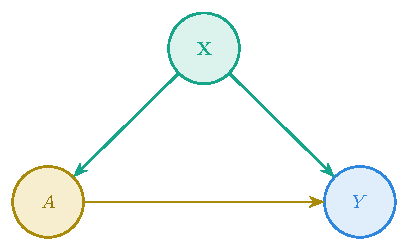
\includegraphics[width=\linewidth]{figures/build/simple_dag.pdf}
\caption{A simple causal DAG with treatment $A$, outcome $Y$, and confounder $X$. The confounder $X$ is a common cause of both the treatment $A$ and the outcome $Y$, which can lead to confounding bias if not properly adjusted for.}
\end{subfigure}

\vspace{0.6cm}

\begin{subfigure}{0.8\textwidth}
\centering
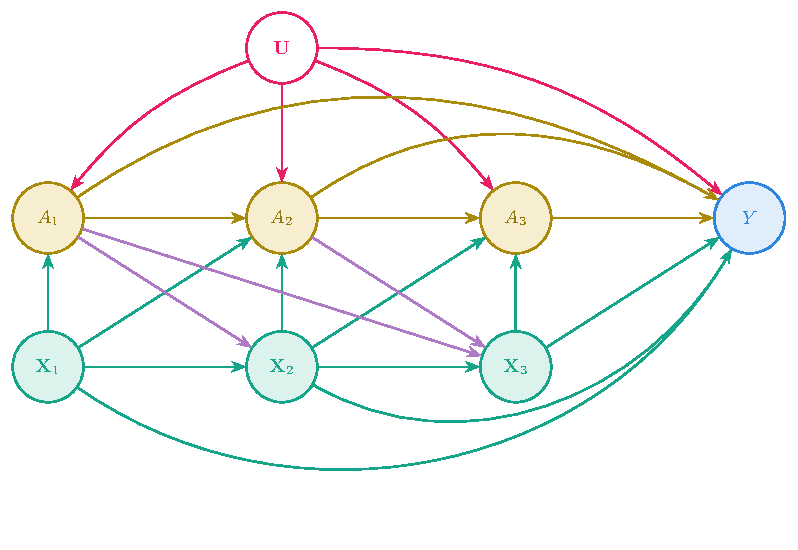
\includegraphics[width=\linewidth]{figures/build/treatment_covariate_feedback.pdf}
\caption{A longitudinal causal DAG with time-varying treatments $A_t$, time-varying confounders $X_t$, and an unobserved confounder $U$.
Filled nodes represent observed variables, while the unfilled node represents an unobserved variable. Arrows 
from $A_t$ to $X_{t+1}$ represent treatment-confounder feedback, where the treatment at time $t$ can affect the confounders at later time points.}
\end{subfigure}

\caption{Two examples of causal DAGs. The first DAG (a) represents a simple static setting with a single treatment and outcome, while the second DAG (b) represents a more complex longitudinal setting with time-varying treatments.}
\label{fig:sample_dags}
\end{figure}

 

and the second dimension is the presence or absence of such feedbacks.
To situate the two methods that we are going to compare in this thesis, we will review 
There are different suggested identification strategies for specifically designed to address such feedbacks such as the g-formula or inverse probability of treatment weighting (IPTW) \cite{robinsEstimationCausalEffects2008a}. 
However, these identification strategies rely on the assumption of 
sequential ignorability, which states that the researcher 
has gathered all the \emph{required} data for the causal analysis or more  
formally there are no unmeasured confounders between the treatments and the outcome at each time point. %In the most general case, 
%confounders can be seen as a common cause of two or more variables in the causal graph. 
%In the context of longitudinal data, we are often concerned about unmeasured confounders effecting the 
%treatment assignment and the outcome at each time point.  
This is a strong assumption and often violated in real world settings. 

To address the problem of unmeasured confoundedness in static settings, there have been 
different methods proposed. Some need additional data with a very specific 
structure such as instrumental variable methods \cite{angristIdentificationLocalAverage1996} 
or using proxy variables \cite{tchetgenIntroductionProximalCausal2020}, 

while others rely on strong assumptions about the data generating process such as the deconfounder method \cite{wangBlessingsMultipleCauses2019}.